\documentclass[10pt]{article}
\usepackage[margin=1cm]{geometry}
\usepackage[portuguese]{babel}
\usepackage[utf8]{inputenc}
\usepackage{hyperref}
\usepackage{indentfirst}
\usepackage{subfig}
\usepackage{listings}
\usepackage{color}
\usepackage[export]{adjustbox}

\definecolor{dkgreen}{rgb}{0,0.6,0}
\definecolor{gray}{rgb}{0.5,0.5,0.5}
\definecolor{mauve}{rgb}{0.58,0,0.82}
\definecolor{codegreen}{rgb}{0,0.6,0}
\definecolor{codepurple}{rgb}{0.58,0,0.82}

\lstdefinestyle{mystyle}{
  commentstyle=\color{codegreen},
  % keywordstyle=\color{magenta},
  % stringstyle=\color{codepurple},
  basicstyle=\ttfamily\footnotesize,
  breakatwhitespace=false,
  breaklines=true,
  captionpos=b,
  keepspaces=true,
  numbers=left,
  numbersep=5pt,
  showspaces=false,
  showstringspaces=false,
  showtabs=false,
  tabsize=2
}
\lstset{style=mystyle}

\urlstyle{same}
\pagenumbering{gobble}
%\usepackage{multicol}
\hypersetup{
  colorlinks=true,
  linkcolor=black,
  filecolor=magenta,      
  urlcolor=blue,
  citecolor=black,
}
\usepackage[backend=bibtex]{biblatex}
\usepackage{graphicx}
\usepackage{tikz}
\pagestyle{plain}

\newcommand{\gaspar}{Diogo Gaspar, 99207}

\begin{document}
\begin{center}
{\huge{Exercício 10 - Projeto Computacional PE 2022}} \\
\vspace{1.5mm}
{\large{\gaspar}} \\
\end{center}

Consideremos como premissas que foram fixadas uma semente em 301 e um conjunto de
tamanhos de amostras \{100, 200, ..., 2500\}.
O objetivo deste exercício passa por gerar 800 amostras com distribuição exponencial
de valor esperado $\frac{1}{\lambda} = \frac{1}{3.13}$ para cada tamanho supra-mencionado.
De seguida, substituir 25\% das observações de cada amostra por outras geradas de uma
população que modela a distribuição dos \textit{outliers}, tal que $\lambda_c = 0.53$.
Para cada amostra, construir um intervalo de confiança para o inverso do valor esperado,
com nível de confiança $1 - \alpha = 0.94$. 
Por fim, para cada tamanho de amostra (contaminada e não contaminada),
calcular a média da amplitude de todos os intervalos de confiança obtidos.
Para tal, recorreu-se ao seguinte trecho de código \texttt{R} (utilizando as bibliotecas \texttt{ggplot2, dplyr} e \texttt{tidyr}):

\begin{lstlisting}[language=R]
  set.seed(301)
  m <- 800
  lambda_not_contaminated <- 3.13
  lambda_contaminated <- 0.53
  alpha <- 1 - 0.94
  dimensions <- seq(100, 2500, 100)
  epsilon <- 0.25

  calculate_mean_widths <- function(n) {
    not_contaminated <- c()
    contaminated <- c()
    for (i in 1:m) {
      contaminated_amount <- floor(n * epsilon)
      nc_exp <- rexp(n, rate=lambda_not_contaminated)
      c_exp <- rexp(contaminated_amount, rate=lambda_contaminated)
      c_exp <- c(c_exp[0:contaminated_amount], nc_exp[contaminated_amount:n])

      nc_upper_bound <- ((1 + qnorm(1-alpha/2)/sqrt(n))/mean(nc_exp))
      nc_lower_bound <- ((1 - qnorm(1-alpha/2)/sqrt(n))/mean(nc_exp))
      c_upper_bound <- ((1 + qnorm(1-alpha/2)/sqrt(n))/mean(c_exp))
      c_lower_bound <- ((1 - qnorm(1-alpha/2)/sqrt(n))/mean(c_exp))
      not_contaminated <- c(not_contaminated, abs(nc_upper_bound - nc_lower_bound))
      contaminated <- c(contaminated, abs(c_upper_bound - c_lower_bound))
    }
    return(c(mean(not_contaminated), mean(contaminated)))
  }

  not_contaminated <- c()
  contaminated <- c()
  for (n in dimensions) {
    mean_widths <- calculate_mean_widths(n)
    not_contaminated <- c(not_contaminated, mean_widths[1])
    contaminated <- c(contaminated, mean_widths[2])
  }

  df = data.frame(dimensions, not_contaminated, contaminated)
  df <- rename(df, "Não Contaminado" = "not_contaminated", "Contaminado" = "contaminated")
  df <- pivot_longer(df, "Não Contaminado":"Contaminado")
  df <- rename(df, "Amostra" = name, mean_widths = value)

  ggplot(df, aes(x = dimensions, y = mean_widths, colour = Amostra)) +
    geom_line() +
    geom_point() +
    labs(x = "Dimensão da Amostra", y = "Amplitude média para 800 amostras") +
    ggtitle("Amplitude média dos intervalos de confiança da distribuição exponencial") +
    theme_bw() +
    scale_colour_brewer(palette = "Set1") +
    theme(axis.text.x = element_text(angle = 40, hjust=1))
\end{lstlisting}

\begin{tikzpicture}[remember picture, overlay]
  \node [shift = {(-4cm, -9.25cm)}] at (current page.north east)
    { 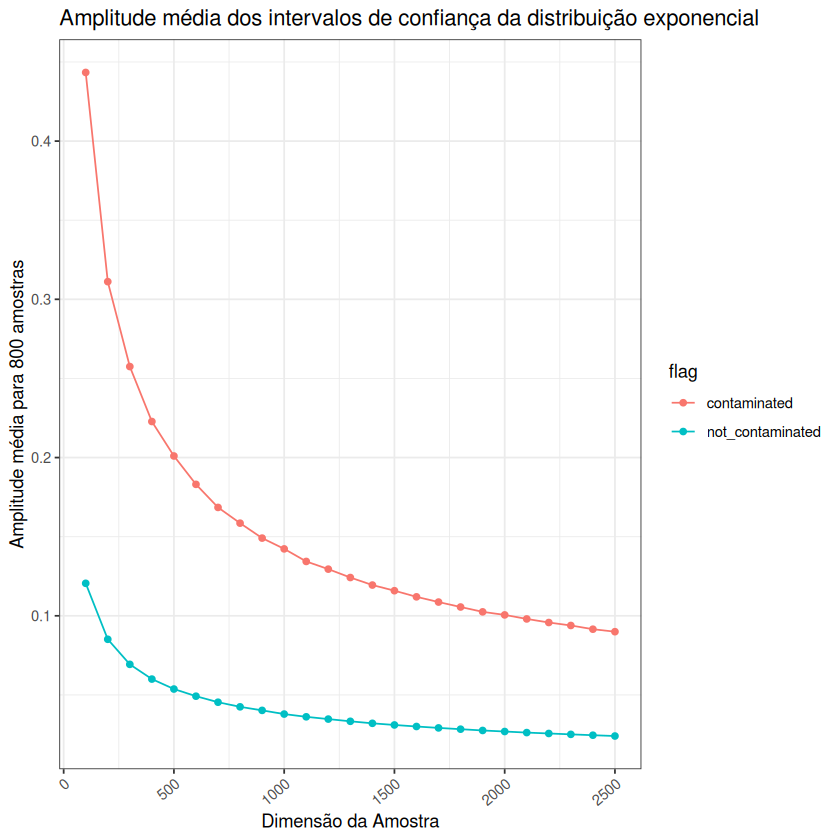
\includegraphics[scale = 0.4]{../imgs/exercise-10.png} };
\end{tikzpicture}

Note-se que ambas as curvas, para amostras não contaminadas e contaminadas,
seguem destinos semelhantes: começam relativamente elevadas, começam a decrescer muito
rapidamente, eventualmente acabando por começar a estabilizar próximo de 1500, até 2500. Mais, note-se que amostras
com indivíduos não contaminados apresentam amplitude média razoavelmente maior, levando
portanto à conclusão de que amostras com indivíduos contaminados têm maior grau de confiança,
com $\lambda > \lambda_c$.

\end{document}